%情報処理学会全国大会原稿テンプレート ver. 1.2

%2段落にするためにtwocolumnを追加
\documentclass[uplatex,twocolumn]{jsarticle}
\usepackage[top=30mm,bottom=25mm,left=20mm,right=20mm]{geometry}
\usepackage[T1]{fontenc}
\usepackage{txfonts}
\usepackage{wrapfig}
\usepackage[expert,deluxe]{otf}
\usepackage[dvipdfmx,hiresbb]{graphicx}
%ハイパーリンクに色がつかないようにするため、hidelinksを追加
\usepackage[dvipdfm]{hyperref}
\usepackage{pxjahyper}
%2段落にするために以下を追加
\usepackage{multicol}
\setlength{\columnsep}{7mm}

\makeatletter
  \renewcommand{\section}{%
    \if@slide\clearpage\fi
    \@startsection{section}{1}{\z@}%
    {\Cvs \@plus.5\Cdp \@minus.2\Cdp}% 前アキ
    {.5\Cvs \@plus.3\Cdp}% 後アキ
    %{\normalfont\Large\headfont\raggedright}}
    {\normalfont\raggedright}}

  \renewcommand{\subsection}{\@startsection{subsection}{2}{\z@}%
    {\Cvs \@plus.5\Cdp \@minus.2\Cdp}% 前アキ
    {.5\Cvs \@plus.3\Cdp}% 後アキ
    %{\normalfont\large\headfont}}
    {\normalfont}}

  \renewcommand{\subsubsection}{\@startsection{subsubsection}{3}{\z@}%
    {\Cvs \@plus.5\Cdp \@minus.2\Cdp}%
    {\z@}%
    %{\normalfont\normalsize\headfont}}
    {\normalfont}}
    
  %2段落で画像貼り付けをするために以下を追加    
  \newenvironment{figurehere}
    {\def\@captype{figure}}
    {}      
    
\makeatother
%ここから上を編集する必要はない.





\title{\vspace{-10mm}大学入試センター試験数学Ⅰ・Aを用いた数式処理システムの性能評価 \footnotemark[0]}
\author{森谷 慧士 \footnotemark[2]\qquad 矢吹 太朗  \\ 千葉工業大学 社会システム科学部 プロジェクトマネジメント学科\footnotemark[2]}
\date{}%日付を入れる必要はない.
\pagestyle{empty}%ページ番号は振らない.
\begin{document}
\twocolumn[\maketitle]

%脚注の追加をするために以下を追加
\begingroup
\def\thefootnote{\fnsymbol{footnote}}
\footnotetext[0]{Performance evaluation of symbolic computation system in solving National Center Test for University Admissions math problems.}%要修正(最後はピリオド)
\footnotetext[2]{Satoshi Moriya(s1242116nc@s.chibakoudai.jp)}%要修正
\footnotetext[3]{Department of Project Management, Faculty of Social Systems Science, Chiba Institute of Technology.}
\endgroup




\section{序論}


 
東京大学の入試問題を全自動で解くプロジェクト(東ロボプロジェクト)が進められている\cite{arai2014}.その処理システムは,センター試験の模擬試験(5教科8科目)で950満点中511点(偏差値は57.8)を獲得,数学と世界史の偏差値は特に高く,数学Ⅰ・A は偏差値64,数学Ⅱ・Bは偏差値65.8,世界史は偏差値66.5だっという\cite{tourobo}.

人工知能がこのように発達すると,その影響は数学教育にも及ぶだろう.今日の数学教育は,すべてを紙と鉛筆で行うことを前提に行われているが,その一部は コンピュータで置き換えることができるはずである.人間が行うこととコンピュータが行うことをうまく識別する能力の育成が求められるようになるだろう.

数式処理を行う人工知能も存在する.Wolfram社が開発したMathematicaである.

Mathematica とは,あらゆる分野の計算に対応する豊富な関数と高度なグラフィック機能を備えた数式所為システムである.Mathematica を提供しているウルフラム・リサーチ社を創業したスティーブン・ウルフラム氏が考案し広く使われている数式処理システムである\cite{wolfram2014}.

Mathematica は,Wolfram 言語を利用する.

Wolfram 言語とは,ウルフラム・リサーチ社が開発した,非常に汎用性の高いマルチパラダイムプログラミング言語である.
Wolfram 言語は,Mathematica 独自のノートブックインターフェイス上で利用することで,インタラクティブなデータ処理を行うスクリプトとして利用できる.さらに,アプリケーションの開発言語として利用すれば,GUI から高度な計算エンジンまで,一貫して一つの環境下で開発を行うことが出来る.

Wolfram 言語は,汎用的なデータベースやインターネット上のデータを直接取り組むことができ,5000 もの組み込み関数を内蔵しているため,わずか数行でも高度なアプリケーションも開発できる.また,Wolfram言語はMathematica だけでなくWolfram 社が無償で提供しているWolfram Alpha でも利用できる\cite{mitubisi}.



\section{目的}

本研究では,大学入試センター試験数学I・Aを題材にして,数学教育にコンピュータを導入することの可能性を調査する.その結果として,高校程度の数学能力を問う問題をコンピュータを活用して解く際に必要となる数学の知識とコンピュータの知識を明らかにすることを目指す.





\section{手法}


 
本研究では大学入試センター試験の数学にMathematicaを用いて解く.そして,使用したコードの数と,利用した数学的知識を集計する.
大学入試センター試験の問題は,紙と鉛筆だけで解けるように作られているため,そこにコンピュータを導入してももちろん解ける.そこで本研究では,問題をそのまま素直に解釈して,Mathematicaで解くようにする.

第一工程では,大学入試センター試験の数学の問題をできるだけ人間が頭を使わずに,素直に数学的表現に翻訳する.
第二工程では,第一工程で数学的表現に翻訳した式をMathematica に与えて数式処理を行う.この工程では,Mathematica が式を最適に処理できるコードを与えて,最適解を得る.この際に,使用したコードの種類を集計し,統計を取る.

例えば,「二次関数\[3a^2 -6a-36=-27\]を解け」という問題を解く.この問題には,Solveというコードを用いる.このSolveは,方程式の解を求めるのに用いられる.\[Solve[3a^2 -6a-36==-27,a]\]とMathematicaに打ち込み,解かせると,\[{{a \rightarrow -1},{a \rightarrow 3}}\]という答えが帰ってくる.

次に,「二次不等式\[2a^2 -6a-36 \le 0\]を解け」という問題を解く.この問題には,Reduceというコードを用いる.このReduceは,方程式あるいは不等式を解き,限定子を除去することで命題を簡約する.\[Reduce[2a^2 -6a-36 \le 0,a]\]とMathematicaに打ち込むと,\[-3 \le a \le 6\]という答えが帰ってくる.
例のように,問題に対して的確なコードを探しだし,Mathematicaを用いて解くという方法を用いる.
試験の年数を重ねることで,新しく使用するコードの種類が減少し,新しくコードを増やすことがなくなると考える.



\section{結果}

\begin{figure}[!htb]
\centering
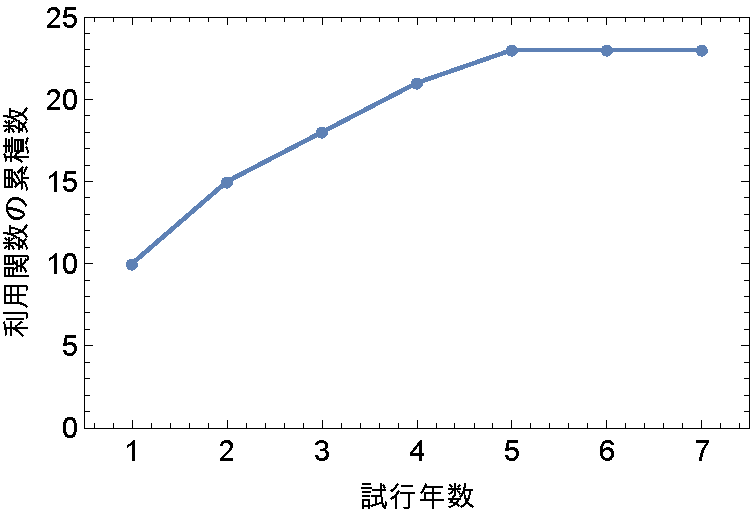
\includegraphics[width=7cm]{code.pdf}
\caption{試行年数に対する使用関数の累積数}\label{サンプル図}
\end{figure}

現在までに,2009~2015年までのセンター試験の数学1・A をMathematicaに処理させた.そして,処理したコードが2年連続して新たに現れることがなくなったため,調査を終了し統計を取ることにした.

図1より,使用したコードはSolveやReduceの使用回数が最も多く,その他
\[Simplify,SolveAlways,Maxmize,TrigExpand,TrigFactor\]
\[TigReduceFactorInteger,Divisors,Length,Sqrt,!,Clear\]
\[Integate,Factor,Cos,Sin,f[x_],Expand,HornerForm,Degree\]の合計23種類となった.



\section{考察}

以上の結果より,人工知能であるMathematicaにセンター試験の数学Ⅰ・Aを解かせる際に使用数コードは,一定数となることがわかる.
これは,年度ごとに出題される問題の種類が違うが,問題内容が似ているため使用するコードも同じものを使用したと考える.
また,出題される問題の種類の統計を取ると,年度ごとに出題される範囲が異なるものもあるが,「整数の性質」や,「場合の数・確率」といった問題範囲は,すべての年度で出題されるので,これらの問題に関しては,各年度で同じコードを反復して使用したと考える.

\section{結論}
本研究では,Mathematicaを用いて大学入試センター試験1・Aを処理させ,数式処理システムの性能評価を実施した.評価するには調査年数が少ないことは否めないが,7年分の調査でも十分評価することは可能である.




\bibliographystyle{junsrt}
\bibliography{biblio}%「biblio.bib」というファイルが必要.

\end{document}